% Metódy inžinierskej práce

\documentclass[10pt,twoside,english,a4paper]{article}

\usepackage[english]{babel}
%\usepackage[T1]{fontenc}
\usepackage[IL2]{fontenc} % lepšia sadzba písmena Ľ než v T1
\usepackage[utf8]{inputenc}
\usepackage{graphicx}
\usepackage{url} % príkaz \url na formátovanie URL
\usepackage{hyperref} % odkazy v texte budú aktívne (pri niektorých triedach dokumentov spôsobuje posun textu)

\usepackage{cite}
%\usepackage{times}

\pagestyle{headings}

\title{Benefits of Implementing Gamification in Health \& Well being and the Ethics behind It\thanks{Semester project in the subject Methods of engineering work, ac. year 2022/23, leading: Fedor Lehocki}} % meno a priezvisko vyučujúceho na cvičeniach

\author{David Truhlar\\[2pt]
	{\small Slovak University of Technology in Bratislava}\\
	{\small Faculty of Informatics and Information Technologies}\\
	{\small \texttt{xtruhlar@stuba.sk}}
	}

\date{\small 05/10/2022} % upravte



\begin{document}

\maketitle

\begin{abstract}
The use of game elements in real-life context for different non-game purposes is increasingly popular today and the gamification of Health and Wellbeing is not an exception. Gamified apps have enormous potential to motivate people to move and exercise regularly, simplify bureaucratic processes, or help educate medical staff in their areas of practice. Yet gamification of healthcare carries potential risks and ethical questions about privacy and misuse of medical records to name just a few. This article will discuss the positive impacts as well as drawbacks of gamification and provide final conclusions.
\end{abstract}

%
%
%

\section*{Introduction}
"Gamification", known as using game elements and techniques  in non-game contexts to motivate and increase user activity \cite{Gamefulness} has become very popular in last decade. These elements are features as levels, rewards, earning points and badges or position in leader-boards. This topic instantly initiated public debate and every industry ranging across productivity, finance, education, news etc. \cite{Gamefulness} started implementing these ideas in their field. The social networks as Facebook or Instagram and other similar platforms, have also contributed to an increase in using of "gamification", in order to improve interaction and engagement with their users. 

Using '"gamified" apps and features in health  has become as popular as  in any other area, and is even becoming today's standard. The badges awarded often aim to encourage health activities and help people to live healthier life-style. The pandemic of Covid-19 has also changed the way we are looking on the implementation of these principles in the real word in terms of education and training of the medical stuff.  Although the research on benefits of these principles is extensive, gamification in health bears many risks that need further discussion. Luckily, these challenges are of ethical character which means their elimination should be achievable by focusing on the human-factor problem.

The concept of gamification can be described in three steps \cite{6758978}. Motivation via implementing gamified elements, psychological outcome - how brain react to the stimulus from the elements, and behavioral outcome - user trying to achieve the goals of the app. These three steps are shown at the Figure~\ref{f:figure1}.

\begin{figure*}[tbh]
\centering
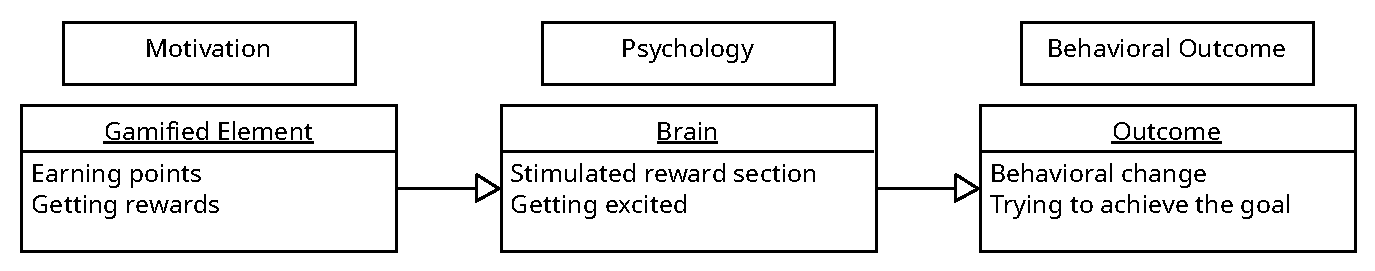
\includegraphics[width=1.0\linewidth]{Figure1.pdf}
\caption{How gamification works.}
\label{f:figure1}
\end{figure*}


Now, the meaning of "gamification" in health will be addressed \ref{G-i-H} and subsequently related benefits will be discussed in section ~\ref{benefits} . In section \ref{risks} risks and possible dangers connected to "gamification" will be examined. Finally, potential solutions for the challenges will be reviewed \ref{solutions} and final conclusions will be made  in summary. ~\ref{summary} .

%
%
%

\section{"Gamification" in health} \label{G-i-H}
Generally, the main goal of "gamified" elements in the context of health and well-being is changing user's behavior by increasing their activity and and/or practicing healthier life-style via game-like experience. The main reason why "gamification" is so popular in last years is strongly linked with the accessibility of digital technologies, particularly smart phones, as well as the created digital infrastructure\cite{Ethics} that has connected the world. 

Gamified elements in general aims at users attention span, in which he is focused on completing the tasks defined by the programmer. The motivation is triggered once the user start collecting the badges for completed goals, and their position in leader-board is getting higher. This type of motivation is similarly applicable to mental health exercises or basic daily tasks including reminders to drink enough water, take one's pills or keep track of the sleep routine. 

The health trackers and health apps have millions of users today, and the competition in this field is enormous. In "Global Healthcare Gamification Market Analysis and Trends - Industry Forecast to 2025", research conducted by Research and Markets, the estimated market gap for "gamification" in healthcare is expected to reach \$13.58 billion by 2025 \cite{mgap} .  

Apple is one of the most significant examples of companies that implemented gamified elements successfully in their market strategies. The ecosystem created between user's Apple Watch and iPhone where user is rewarded for accomplishing tasks connected to movement - steps, calories and the count of hours user was active is one of the most used practice \cite{aboveAvalon} of gamification in terms of behavioral change and motivation.  Apple also rewards people on special days. For example, on the Earth Day (April 22.) the user can get a 'special' badge for exercising more than 30 minutes in that day\cite{earthDay}. 

Next, the benefits of gamifiaction in health will be discussed.

%
%
%

\section{Benefits} \label{benefits}
The concept of implementing game-like element in different areas of healthcare and well being has been talked about for some years and there are companies that managed to implement them successfully. This implementation opens up many ways to encourage users to be involved with their own health.  

\subsection{Helthier life-style } \label{lifestyle}
-Strava App
-Apple Watch
-Sweatcoin

\subsection{Educated medical stuff} \label{stuff}
-Simulators
-Online courses

\subsection{Reducing bureaucratic processes} \label{bureau}
-Papers can be stored online
-databases instead of offices
-medical records online

%Základným problémom je teda\ldots{} Najprv sa pozrieme na nejaké vysvetlenie (časť), a potom na ešte nejaké (časť.\footnote{Niekedy môžete potrebovať aj poznámku pod čiarou.}

%Môže sa zdať, že problém vlastne nejestvuje, ale bolo dokázané, že to tak nie je. Napriek tomu, aj dnes na webe narazíme na všelijaké pochybné názory.% Dôležité veci možno \emph{zdôrazniť kurzívou}.

%
%
%

\section{Risks} \label{risks}
Ethical questions..

\subsection{Privacy}\label{privacy}
-privacy policy problems

\subsection{Medical records} \label{records}
-Misuse of medical records

\subsection{Addiction} \label {addiction}
-People can get addicted on awards - dopamine

%
%
%

\section{Possible solutions} \label{solutions}

%
%
%

\section{Summary} \label{summary} % prípadne iný variant názvu

%
%
%

%\section{ priklady zo vzoru}\label{priklady}
 %Niekedy treba uviesť zoznam:

%\begin{itemize}
%\item jedna vec
%\item druhá vec
%	\begin{itemize}
%	\item x
%	\item y
%	\end{itemize}
%\end{itemize}

%Ten istý zoznam, len číslovaný:

%\begin{enumerate}
%\item jedna vec
%\item druhá vec
%	\begin{enumerate}
%	\item x
%	\item y
%	\end{enumerate}
%\end{enumerate}

%\acknowledgement{Ak niekomu chcete poďakovať\ldots}

%\paragraph{Veľmi dôležitá poznámkaNiekedy je potrebné nadpisom označiť odsek. Text pokračuje hneď za nadpisom.


% týmto sa generuje zoznam literatúry z obsahu súboru literatura.bib podľa toho, na čo sa v článku odkazujete
\bibliography{lit1}
\bibliographystyle{plain} % prípadne alpha, abbrv alebo hociktorý iný
\end{document}
